% !TEX root = ../main.tex
\section{Q09: Optimale valg av medarbeideres innsats -- agentens og prinsipalens side}\label{q:09}

\begin{quote}
\emph{Vis og forklar modellerne der anviser optimale valg af medarbejderes indsats -- set både fra medarbejderens (agentens) side og virksomhedens (principalens) side. Diskuter forhold som: a) risiko, b) præstationsuafhængig løn, c) incitamentskoefficienter.}
\end{quote}

\subsection*{Svar (kort)}
Spørsmålet besvares med den lineære principal-agent-modellen: output $Q=\alpha e+\mu$ (innsats $e$ ganger produktivitet $\alpha$, pluss støy $\mu$) og lønn $W=W_0+\beta Q$ (fastlønn $W_0$ pluss en andel $\beta$ av resultatet). \emph{Agenten} velger innsats $e^{*}$ slik at marginalt insentiv $\beta\alpha$ er lik marginal innsatskostnad $c'(e)$ -- altså arbeider hun helt til ekstra kroner fra bonus akkurat dekker ekstra slit. \emph{Prinsipalen} velger insentivkoeffisienten $\beta^{*}=1/(1+r\sigma^{2}c''/\alpha^{2})$. Intuitivt: jo høyere risikoaversjon ($r$) eller støy ($\sigma^{2}$), jo lavere bør $\beta$ settes -- fordi det blir dyrt å lesse risiko over på en risikoavers agent. (a) Risiko ($r$, $\sigma^{2}$) trekker $\beta^{*}$ ned; (b) den prestasjonsuavhengige $W_0$ vrir \emph{ikke} innsats, men dekker deltakelseskravet (IR -- Individual Rationality, dvs.\ at jobben må være verdt det) pluss risikopremie; (c) $\beta$ er det eneste insentivverktøyet som faktisk vrir innsats. [SLIDE]

\subsection*{De to modellene (oversikt)}

\begin{center}
\renewcommand{\arraystretch}{1.15}
\begin{tabular}{@{}p{2.8cm}p{3.6cm}p{4.4cm}p{4.6cm}@{}}
\toprule
\textbf{Side} & \textbf{Beslutningsvariabel} & \textbf{Mål} & \textbf{Optimum (FOC)} \\
\midrule
Agent & Innsats $e$ & Max $\mathbb{E}[W]-\tfrac{r}{2}\mathrm{Var}[W]-c(e)$ & $\beta\alpha=c'(e^{*})$ \\
Prinsipal & Kontrakt $(W_0,\beta)$ & Max $\mathbb{E}[Q-W]$ s.t.\ IR + IC & $\beta^{*}=\dfrac{1}{1+r\sigma^{2}c''/\alpha^{2}}$ \\
\bottomrule
\end{tabular}
\end{center}

\subsection*{Relevante teorier (kort)}

\paragraph{\thref{optimal-effort-model}{Optimal effort-modell (begge sider)}\quad\STwo/\SThree}
Modellen i BSZ kap.\ 15: output $Q=\alpha e+\mu$ (det agenten produserer), kontrakt $W=W_0+\beta Q$, og en konveks innsatskostnad $c(e)$ -- ``konveks'' fordi siste innsats-time gjør mer vondt enn første. Agentens FOC -- førsteordensbetingelsen, dvs.\ regelen for hva som maksimerer agentens nytte -- er $\beta\alpha=c'(e^{*})$. Sagt enkelt: agenten jobber til marginal bonus akkurat dekker marginal slit. Innsats er derfor strengt stigende i $\beta$ (mer bonus $\Rightarrow$ mer innsats) og uavhengig av $W_0$ (fastlønn endrer ikke marginalvurderingen). Prinsipalen tar agentens beste respons med i regnestykket og velger $\beta^{*}$ der marginal insentivgevinst er lik marginal risikopremie. Modellen leverer dermed begge optimumsbetingelsene i samme ramme og forklarer hvorfor \emph{second-best} -- nest-beste utfall, dvs.\ det beste man får når innsats ikke kan observeres -- har $\beta<1$. [SLIDE]

\paragraph{\thref{fixed-vs-variable-pay}{Prestasjonsuavhengig lønn ($W_0$) vs.\ variabel ($\beta Q$)}\quad\SThree}
$W_0$ er en ren \emph{nivå}-variabel: den løfter hele lønnsnivået og oppfyller deltakelsesskranken (IR -- jobben må gi minst like mye nytte som beste alternativ), og kompenserer agenten for risikopremien $\tfrac{r}{2}\beta^{2}\sigma^{2}$. Den vrir \emph{ikke} marginal innsats, fordi $W_0$ utbetales uansett hva agenten gjør. $\beta Q$ er derimot en ren \emph{marginal}-variabel: hver ekstra produserte enhet gir mer bonus, så innsats vris -- men risiko fra støyen $\mu$ overføres til agenten. Bare $W_0$ (uten bonus) gir \emph{shirking} (lav innsats / lureri); bare $\beta Q$ (uten fastlønn) gir ineffektiv risikodeling. Hybridkontrakter er derfor normen: $W_0$ håndterer deltakelse og risiko, $\beta Q$ håndterer innsats. [SLIDE]

\paragraph{\thref{incentive-coefficient}{Insentivkoeffisient $\beta=\partial W/\partial Q$}\quad\SThree}
$\beta$ måler ``pay-performance sensitivity'' (lønnsfølsomhet for resultat) -- hvor mange ekstra kroner lønn én ekstra krone resultat gir. Determinanter: $\beta^{*}$ stiger med produktivitet $\alpha$ (sterkere kobling mellom innsats og output $\Rightarrow$ mer å hente på å gi bonus); $\beta^{*}$ faller med risikoaversjon $r$, støy $\sigma^{2}$ og kostnadens konveksitet $c''$ (jo brattere kostnadskurven blir, jo mindre ekstra innsats får man uansett). Empirisk varierer $\beta$ fra omtrent $0$ (tariffstillinger som sykepleier) til omtrent $1$ (\emph{franchising} -- der franchisetaker eier hele residualen, og \emph{residual claimancy} betyr at agenten beholder alt overskudd). Holmström--Milgrom (1991): hvis agenten har flere oppgaver der bare én er målbar (\emph{multitasking}), må $\beta$ senkes -- ellers vil agenten dumpe de umålbare oppgavene og bare jobbe med det som teller på bonusen. [SLIDE]

\paragraph{\thref{risk-sharing}{Risikodeling}\quad\SThree}
Risikoavers agent + diversifisert risikonøytral prinsipal (en eier som spør lite om risiko, fordi formuen er spredt) $\Rightarrow$ \emph{Pareto-optimal} (ingen kan bli bedre stilt uten at noen blir verre stilt) risikodeling tilsier first-best, dvs.\ ren fastlønn til agenten -- eieren bærer all risikoen. Men da forsvinner insentivet til å jobbe. Second-best krever at agenten bærer \emph{noe} risiko gjennom $\beta>0$, og prinsipalen må kompensere med en risikopremie. Risikopremien $\tfrac{r}{2}\beta^{2}\sigma^{2}$ -- som intuitivt sier at risikokostnaden vokser med kvadratet av $\beta$ og lineært med agentens risikoaversjon og støyen -- er kjernen i \thref{agency-costs}{agency costs} (kostnaden ved at agenten ikke kan bli direkte styrt) i denne modellen. Når $\sigma^{2}$ er stor, brukes \thref{informativeness-principle}{informativeness-mekanismer} -- altså tilleggssignaler som filtrerer bort eksogen støy -- som relative måltall, peer-grupper og indekserte opsjoner. [SLIDE]

\subsection*{Illustrasjoner fra forelesning}

\begin{figure}[H]
  \centering
  
\includegraphics[width=0.4\linewidth]{BSZ_kap_15_2026/by_slide/slide_002/BSZ_kap_15_2026_slide_002_asset_01_image1.png}
  \caption{Insentivkompensasjon: agenten responderer på $\beta$ -- høyere pay-performance sensitivity gir sterkere innsats, men krever risikopremie. (BSZ kap.\ 15, slide 2) [SLIDE]}
\end{figure}

\subsection*{Grafisk modell -- to bilder (agent + prinsipal)}

\begin{figure}[H]
\centering

\includegraphics[width=0.55\linewidth]{BSZ_kap_15_2026/by_slide/slide_014/BSZ_kap_15_2026_slide_014_asset_01_image3.png}
\caption{Pensumets versjon av principal-agent-modellen: $Q=\alpha e+\mu$ og $W=W_0+\beta Q$. [SLIDE -- BSZ kap.\ 15, slide 14]}
\end{figure}

Agentens side kan tegnes på to måter, som henger sammen som ``totalbildet'' og ``marginalbildet'' av samme optimum: (1) \emph{totalkurver} -- kompensasjon $W=W_0+\beta\alpha e$ som rett linje og kostnad $c(e)=e^{2}$ som konveks kurve, hvor $e^{*}$ er der tangenten til kostnadskurven er parallell med kompensasjonslinjen; (2) \emph{deriverte kurver} -- $MB=\beta\alpha$ horisontal og $MC=c'(e)=2e$ stigende, hvor $e^{*}$ er rett krysningspunkt. Det er samme FOC ($\beta\alpha=c'(e^{*})$), bare lest ut av to forskjellige grafer.

\begin{figure}[H]
\centering
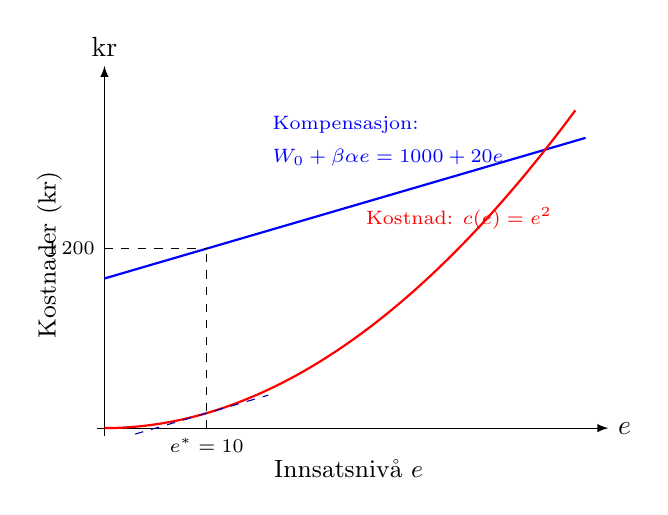
\begin{tikzpicture}[>=latex]
  % Skalafaktorer: 1 effort-enhet = 0.13 cm, 1 kr = 0.0019 cm
  % Akser (i cm)
  \draw[->] (-0.1,0) -- (6.4,0) node[right] {$e$};
  \draw[->] (0,-0.1) -- (0,4.6) node[above] {kr};
  \node[below=8pt] at (3.1,0) {\small Innsatsnivå $e$};
  \node[rotate=90] at (-0.7,2.2) {\small Kostnader (kr)};
  % Kompensasjonslinje W = 1000 + 20e (cm: x=e*0.13, y=W*0.0019)
  \draw[thick,blue] (0,1.9) -- (6.11,3.686);
  \node[blue,above,align=left] at (3.6,3.2) {\scriptsize Kompensasjon:\\ \scriptsize $W_0+\beta\alpha e=1000+20e$};
  % Kostnadskurve c(e) = e^2
  \draw[thick,red,domain=0:46,samples=80,smooth]
    plot ({\x*0.13},{\x*\x*0.0019});
  \node[red,above] at (4.5,2.4) {\scriptsize Kostnad: $c(e)=e^{2}$};
  % Tangent ved e*=10 (stigning 20): y = 20e - 100
  \draw[dashed,blue!70!black] (0.39,-0.076) -- (2.08,0.418);
  % Hjelpe-streker for e*=10 og W=1200
  \draw[dashed] (1.3,0) -- (1.3,2.28);
  \draw[dashed] (0,2.28) -- (1.3,2.28);
  \node[left] at (0,2.28) {\scriptsize $1\,200$};
  \node[below] at (1.3,0) {\scriptsize $e^{*}=10$};
\end{tikzpicture}
\caption{\textbf{Agentens side -- totalmodellen (ikke-derivert).} Kompensasjonslinjen $W=W_0+\beta\alpha e$ (her $W_0=1000$, $\beta\alpha=20$) og den konvekse kostnadskurven $c(e)=e^{2}$. Agenten velger $e^{*}=10$ der tangenten til kostnadskurven er parallell med kompensasjonslinjen -- altså $c'(e^{*})=2e^{*}=20=\beta\alpha$. Total kompensasjon ved $e^{*}$: $W=1\,200$. Krever \texttt{\textbackslash usepackage\{tikz\}} i preamble.}
\end{figure}

\begin{figure}[H]
\centering
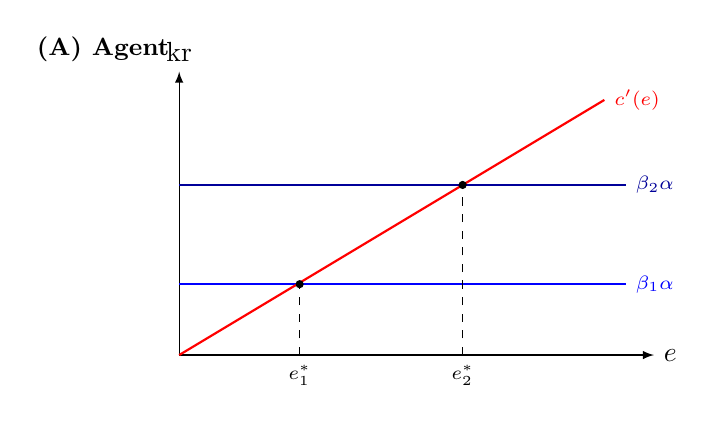
\begin{tikzpicture}[>=latex,scale=0.9]
  % Akser
  \draw[->] (0,0) -- (6.7,0) node[right] {$e$};
  \draw[->] (0,0) -- (0,4.0) node[above] {kr};
  \node[above left] at (0,4.0) {\small \textbf{(A) Agent}};
  % MB-linjer
  \draw[thick,blue] (0,1.0) -- (6.3,1.0) node[right] {\scriptsize $\beta_1\alpha$};
  \draw[thick,blue!60!black] (0,2.4) -- (6.3,2.4) node[right] {\scriptsize $\beta_2\alpha$};
  % MC
  \draw[thick,red] (0,0) -- (6.0,3.6) node[right] {\scriptsize $c'(e)$};
  % Optima
  \draw[dashed] (1.7,0) -- (1.7,1.0); \filldraw (1.7,1.0) circle (1.4pt);
  \node[below] at (1.7,0) {\scriptsize $e_1^{*}$};
  \draw[dashed] (4.0,0) -- (4.0,2.4); \filldraw (4.0,2.4) circle (1.4pt);
  \node[below] at (4.0,0) {\scriptsize $e_2^{*}$};
\end{tikzpicture}\quad
\begin{tikzpicture}[>=latex,scale=0.9]
  % Akser
  \draw[->] (0,0) -- (6.7,0) node[right] {$\beta$};
  \draw[->] (0,0) -- (0,4.0) node[above] {kr};
  \node[above left] at (0,4.0) {\small \textbf{(B) Prinsipal}};
  \draw (5.2,0) node[below] {\scriptsize $1$};
  \draw[dashed] (5.2,0) -- (5.2,3.2);
  % MB(β) konkav
  \draw[thick,blue,domain=0:5.2,samples=60]
    plot (\x,{3.0*(1-exp(-0.7*\x))}) node[right] {\scriptsize $MB(\beta)$};
  % MC(β) konveks
  \draw[thick,red,domain=0:5.2,samples=60]
    plot (\x,{0.35*\x*\x}) node[right] {\scriptsize $MC(\beta)$};
  % Krysning -- MB(2.7)=2.55, MC(2.7)=0.35*7.29=2.55
  \filldraw (2.7,2.55) circle (1.4pt);
  \draw[dashed] (2.7,0) -- (2.7,2.55);
  \node[below] at (2.7,0) {\scriptsize $\beta^{*}$};
\end{tikzpicture}
\caption{\textbf{(A) Agentens side:} $e^{*}$ der $\beta\alpha=c'(e)$; en høyere $\beta$ skifter $MB$ opp og $e^{*}$ til høyre. \textbf{(B) Prinsipalens side:} $\beta^{*}$ der marginal insentivgevinst lik marginal risikopremie $\tfrac{r}{2}\beta^{2}\sigma^{2}$; $\beta^{*}<1$ i second-best. Krever \texttt{\textbackslash usepackage\{tikz\}} i preamble.}
\end{figure}

\textbf{Hvordan de to grafene henger sammen.} Grafene leses sekvensielt: prinsipalen velger $\beta^{*}$ i (B) ved å forutse at agenten vil reagere i (A). Hver verdi av $\beta$ i (B) bestemmer hvor høyt $MB$-linja ligger i (A), og dermed agentens $e^{*}$. Når prinsipalen øker $\beta$, øker insentivgevinsten (mer $e$, mer $Q$) -- men også risikopremien som prinsipalen må betale via $W_0$ for å holde IR. Optimum er der \emph{disse to skråningene treffer hverandre}: avtagende marginalgevinst (konkav $MB$) møter stigende marginal risikokostnad (konveks $MC$). Det er nettopp denne trade-offen som gir Holmström-Milgrom-formelen for $\beta^{*}$ og som forklarer hvorfor $\beta^{*}<1$ alltid med risikoavers agent.

\subsection*{Real-world eksempler}

\textbf{Eks.~1 -- Investment banking-trader vs.\ Statoil/Equinor-toppleder.}\quad [EKS]
Tradere i internasjonale banker har lav $W_0$ (relativt) og høy $\beta$ -- prestasjonen er målbar (P\&L), agenten er typisk lite risikoavers, og produktiviteten ($\alpha$) er stor. I motsetning har Equinor-konsernsjefen en betydelig grunnlønn og en moderat $\beta$ levert via aksjebasert LTI med peer-justering -- fordi oljepris ($\mu$) gir stor støy ($\sigma^{2}$) som må filtreres for at risikopremien ikke skal eksplodere. Samme modell, ulik parametertilstand: traderen sitter ved $\beta\to 1$-enden, Equinor-CEO ved moderat $\beta$.

\textbf{Eks.~2 -- Norsk offentlig sektor vs.\ Aker Solutions provisjons-selger.}\quad [EKS]
Sykepleier i kommunal helse har $\beta\approx 0$, ren tarifflønn: output er svært vanskelig å måle, agenten er risikoavers, og fordelingshensyn favoriserer fastlønn. Aker Solutions selger av offshore-utstyr har $\beta\approx 0{,}3$--$0{,}5$ på kvartals-salgsmål, lavere $W_0$, og bonusen er ``claw-back''-pliktig hvis kunden trekker seg. Sammenligning: identisk modell, men ulike $(\alpha,r,\sigma^{2})$ tvinger fram diametralt motsatte kontrakter. Dette viser at modellen er en \emph{designkalkulator}, ikke en universaloppskrift.

\subsection*{Kobling til Mærsk Power-to-X}
PtX-divisjonens utfall avhenger sterkt av eksogen elektrisitetspris og hydrogen-etterspørsel -- et stort $\sigma^{2}$. Modellen tilsier derfor \emph{lav $\beta$} på topplinjeresultat (EBITDA, NPV) for divisjonsledelsen, fordi å overføre denne risikoen til risikoaverse ledere ville krevd en kostbar risikopremie. Likevel: noe $\beta$ kan kobles til \emph{kontrollerbare milestones} -- anlegg ferdigstilt i tide, OPEX innenfor budsjett, kontrakter signert med PtX-avtakere. Dette er \thref{informativeness-principle}{informativeness-prinsippet} i praksis: bruk de måltall som faktisk signalerer innsats, ikke de som domineres av eksogen støy. Hybridkontrakten (høy $W_0$, lav $\beta$ på finansresultater, moderat $\beta$ på milestones) er Mærsk-konsistent med en risikoavers ledelse i et høy-$\sigma^{2}$-prosjekt. [CASE]

\subsection*{Fallgruber}
\begin{itemize}\setlength{\itemsep}{2pt}
\item Glemme at $W_0$ \emph{ikke} vrir innsats -- klassisk forveksling av nivå og marginal.
\item Anta at høyere $\beta$ alltid er bedre -- ignorerer risikopremien og multitasking.
\item Bare beskrive agentens side uten å vise prinsipalens optimeringsproblem (eller omvendt).
\item Glemme støyen $\mu$ og dens rolle for $\beta^{*}$ -- spørsmålet nevner risiko eksplisitt.
\item Sette $\beta^{*}=1$ uten å forklare at det krever risikonøytral agent eller observerbar innsats.
\item Forveksle insentivproblemet (\thref{moral-hazard}{moral hazard}) med risikodelingsproblemet -- de er separate, men koblet via $\beta$.
\item Tegne MC- og MB-kurvene feil vei (MC stigende, MB i $\beta$ konkav) -- få graf-detaljer galt skader troverdighet.
\end{itemize}

\FloatBarrier
\subsection*{Håndskrivbar disposisjon (15-min forberedelse)}
\begin{itemize}\setlength{\itemsep}{2pt}
\item \textbf{Tese:} To FOC -- agentens for $e^{*}$, prinsipalens for $\beta^{*}$ -- innenfor samme lineære principal-agent-modell.
\item \textbf{Setup:} $Q=\alpha e+\mu$, $W=W_0+\beta Q$, agent CARA + $c(e)$, prinsipal diversifisert.
\item \textbf{Agentside (Modell A):} Max $\mathbb{E}[W]-\tfrac{r}{2}\mathrm{Var}[W]-c(e)\Rightarrow \beta\alpha=c'(e^{*})$. Ian/AssemCo: $e^{*}=50\beta$. \emph{$W_0$ vrir ikke innsats.}
\item \textbf{Prinsipalside (Modell B):} Max $\alpha e^{*}-c(e^{*})-\tfrac{r}{2}\beta^{2}\sigma^{2}\Rightarrow \beta^{*}=\tfrac{1}{1+r\sigma^{2}c''/\alpha^{2}}$.
\item \textbf{(a) Risiko:} $r,\sigma^{2}\uparrow\Rightarrow\beta^{*}\downarrow$. Risikopremien $\tfrac{r}{2}\beta^{2}\sigma^{2}$ er kjernen i agency cost.
\item \textbf{(b) $W_0$:} Faller ut av FOC; rolle = IR + risikopremie-kompensasjon. \emph{Vrir ikke innsats.}
\item \textbf{(c) $\beta$:} Eneste innsatsdriver. Pay-performance sensitivity. Determinanter: $\alpha\uparrow$, $r\downarrow$, $\sigma^{2}\downarrow$ $\Rightarrow$ $\beta\uparrow$.
\item \textbf{Graf A:} $MB=\beta\alpha$ horisontal, $MC=c'(e)$ stigende, kryss = $e^{*}$.
\item \textbf{Graf B:} $MB(\beta)$ konkav, $MC(\beta)=$ risikopremie konveks, kryss = $\beta^{*}<1$.
\item \textbf{Eks.\ 1:} IB-trader (høy $\beta$, lav $W_0$) vs.\ Equinor-CEO (moderat $\beta$, høy $W_0$, peer-justering).
\item \textbf{Eks.\ 2:} Norsk sykepleier (alt $W_0$) vs.\ Aker Solutions selger (provisjon med claw-back).
\item \textbf{Case:} Mærsk PtX -- stort $\sigma^{2}\Rightarrow$ lav $\beta$ på EBITDA, moderat $\beta$ på milestones (\thref{informativeness-principle}{informativeness}).
\item \textbf{Søyle:} \STwo\ + \SThree.
\end{itemize}
